\section{Background}
\label{sec:background}

\subsection{Time Series}

\subsection{Multi-Layer Fully Connected}



\subsection{Recurrent Neural Network}

A Recurrent Neural Network (RNN) is very similar to a feed-forward network, 
except that the connections also links backwards on the network.
So the output is defined similarly to equation \ref{eq:recurrent_net}.
Note that the result from last step contributes to the next and so on,
therefore the $ith$ step depends on all previous steps,
which takes a form of a memory \cite{geron2017hands}.

\begin{equation}
\label{eq:recurrent_net}
Y_{(t)} = \phi(X_{(t)} \dot W_x + Y_{(t-1)} \dot W_y + b)
\end{equation}

The training method analog to the feed-forward networks,
the first step is a forward pass that unroll the network time loop,
the values for all $Y's$ in the time series are also calculated in the process.
The gradient value is calculated using all the results in the cost function,
for example if the time series generates $Y_1, \dots Y_n$ and the cost function uses only the last three values of $Y$,
than the gradient is calculated using only $Y_{n-2}, Y_{n-1} , Y_n$.

Recurrent neural network tends to suffer from exploding and vanishing gradients more than a convolution or fully connected network,
since the number of steps in time it unrolls also adds to the depth of the network.
To solve this problem techniques like batch normalization, non-saturating activation functions and gradient clipping are exploited.

Another problem with the simple approach shown previously happens when the network has to remember inputs far early in the time steps,
most of the information is lost by transversing the network.
To overcome this problem a more sophisticated cell was developed, Long Short Term Memory (LSTM).
The full explanation of how it works is given on subsection \ref{sec:lstm}.
 
\subsection{Long Short Term Memory}
\label{sec:lstm}

The main improvement LSTM cell wants to achieve is learn what to store in the long term memory, what to discard and what to use from the input.
The LSTM cell keeps two state matrix that holds information from previous time sequences,
one for long an the other for short term memory,
those states are than used as input for the next iteration.
The figure \ref{fig:lstm_diagram} show a LSTM diagram, the $c_{(t-1)}$ represents the long term memory input
and the $h_{(t-1)}$ represent the short term memory, note that the short term output is also the $Y_{(t)}$.

The LSTM cell uses one fully connected layer with hyperbolic tangent activation function as the main flow of input
and three other fully connected with logistic activation function as controllers.
Each controller is attached to a gate, basically an element-wise multiplication,
since the logistic function output range is 0 to 1 the gate is either close when 0 or open when 1.

Each gate receives a name based on their function and is controlled by one of the matrix controllers:
\subsubsection{Forget Gate} controls what information from the input is retained on the long term state,
it receives $f_{(t)}$ (logistic function controllers) and $c_{(t-1)}$ (long term state) as input.
\subsubsection{Input Gate} controls which information on the main flow will be added to the long term memory and the output memory,
receives $g_{(t)}$ (main input flow) and $i_{(t)}$ (logistic controller).
\subsubsection{Output Gate} controls the information that goes to the output and short term memory,
receives the addition result from \textit{Input Gate} and \textit{Forget Gate} after an hyperbolic tangent activation function and $o_{(t-1)}$ (logistic function controller).

\begin{figure}
	\centering
	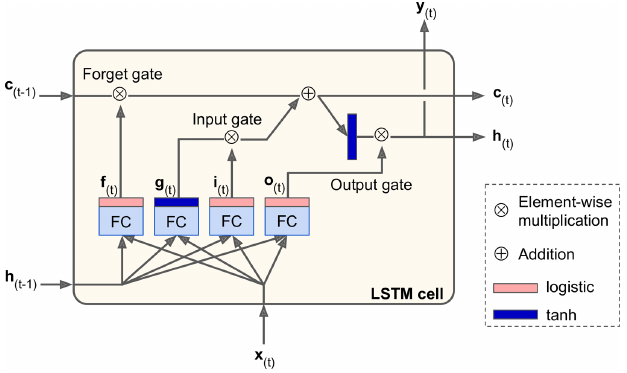
\includegraphics[width=\linewidth]{lstm_diagram.png}
	\caption{LSTM Diagram from \cite{geron2017hands}\label{fig:lstm_diagram}}
\end{figure}



